Penelitian ini dilatarbelakangi oleh keterbatasan sensor LiDAR dua dimensi yang umum digunakan pada robot bergerak otonom untuk navigasi lingkungan dalam ruangan. Meskipun mampu menyediakan informasi jarak secara \textit{real-time} dengan tingkat akurasi yang tinggi, LiDAR 2D hanya melakukan pemindaian pada satu bidang horizontal sehingga objek yang berada di luar bidang tersebut berpotensi tidak terdeteksi (\cite{Fagundes2024,Kibii2022}). Kondisi ini dapat menimbulkan \textit{blind-spot} vertikal yang mengurangi kualitas persepsi lingkungan dan meningkatkan risiko kolisi, khususnya terhadap objek berprofil rendah yang berada di dekat permukaan lantai.

Untuk mengatasi keterbatasan tersebut, penelitian ini mengintegrasikan kamera termal sebagai sensor pelengkap LiDAR. Informasi termal digunakan untuk mengidentifikasi area yang tidak sepenuhnya teramati oleh pemindaian laser sehingga sistem dapat memperoleh representasi lingkungan yang lebih lengkap. Pendekatan integrasi antara LiDAR dan kamera termal telah banyak digunakan untuk meningkatkan robustitas persepsi pada sistem robotika dan kendaraan otonom karena kedua sensor memiliki karakteristik pengamatan yang saling melengkapi (\cite{Choi2023,Schichler2025}). Pada penelitian ini, kedua sensor tidak digabungkan secara langsung pada tingkat data mentah, melainkan diolah menjadi indikator traversability yang menggambarkan tingkat kelayakan lintasan area di depan robot. Nilai traversability dari masing-masing sensor kemudian difusikan untuk menghasilkan informasi kondisi lingkungan yang digunakan pada proses pengambilan keputusan navigasi.

Informasi traversability hasil fusi selanjutnya dimanfaatkan dalam kerangka navigasi ber\-basis \textit{Artificial Potential Field} (APF) (\cite{Khatib1986}). Metode APF dipilih karena memiliki kompleksitas komputasi yang relatif rendah dan mampu menghasilkan respons penghindaran hambatan secara \textit{real-time}. Namun demikian, penggunaan parameter APF yang bersifat tetap sering kali menyebabkan perilaku navigasi kurang adaptif terhadap perubahan kondisi lingkungan (\cite{Lv2024}). Oleh karena itu, penelitian ini memanfaatkan logika fuzzy Mamdani sebagai mekanisme adaptasi parameter navigasi berdasarkan kondisi lingkungan yang diamati sensor. Variabel masukan yang digunakan terdiri atas jarak obstacle terdekat dan nilai traversability efektif hasil fusi sensor, sedangkan keluaran fuzzy berupa skala kecepatan (\textit{speed scale}) dan penguatan gaya tolak (\textit{repulsive gain}) yang digunakan untuk menyesuaikan perilaku APF secara dinamis. Pendekatan serupa telah dilaporkan mampu meningkatkan keamanan dan kelancaran navigasi robot bergerak pada lingkungan yang kompleks (\cite{Haider2022,Benaicha2026}).

Pengembangan dan pengujian sistem dilakukan pada lingkungan simulasi berbasis ROS Noetic dan Gazebo. Penggunaan simulasi dipilih untuk menjamin reproduktivitas eksperimen, mempermudah pengendalian variabel pengujian, serta memungkinkan pelaksanaan percobaan berulang pada kondisi yang identik (\cite{Adiuku2024}). Lokalisasi robot diperoleh melalui \textit{fake\_localization} sehingga posisi robot terhadap peta diketahui secara langsung dan tidak dipengaruhi oleh kesalahan estimasi lokalisasi. Dengan demikian, evaluasi dapat difokuskan pada kinerja sistem navigasi dan kemampuan penghindaran obstacle tanpa dipengaruhi oleh ketidakpastian proses lokalisasi.

Secara umum, penelitian ini dilaksanakan melalui lima tahapan utama yang ditunjukkan pada Gambar~\ref{fig:alur_penelitian}. Tahap pertama adalah studi pendahuluan yang mencakup kajian literatur, identifikasi permasalahan, dan penetapan ruang lingkup penelitian. Tahap kedua adalah perancangan sistem yang meliputi penyusunan arsitektur navigasi, perancangan mekanisme fusi traversability, serta perancangan logika fuzzy Mamdani. Tahap ketiga adalah implementasi seluruh komponen sistem pada lingkungan simulasi. Tahap keempat adalah pelaksanaan eksperimen pada delapan skenario pengujian yang terdiri atas konfigurasi \textit{baseline} dan konfigurasi fuzzy. Tahap terakhir adalah analisis hasil eksperimen menggunakan metrik navigasi yang telah ditentukan untuk mengevaluasi pengaruh integrasi kamera termal, fusi traversability, dan logika fuzzy terhadap performa sistem navigasi robot.

\begin{figure}[H]
\centering
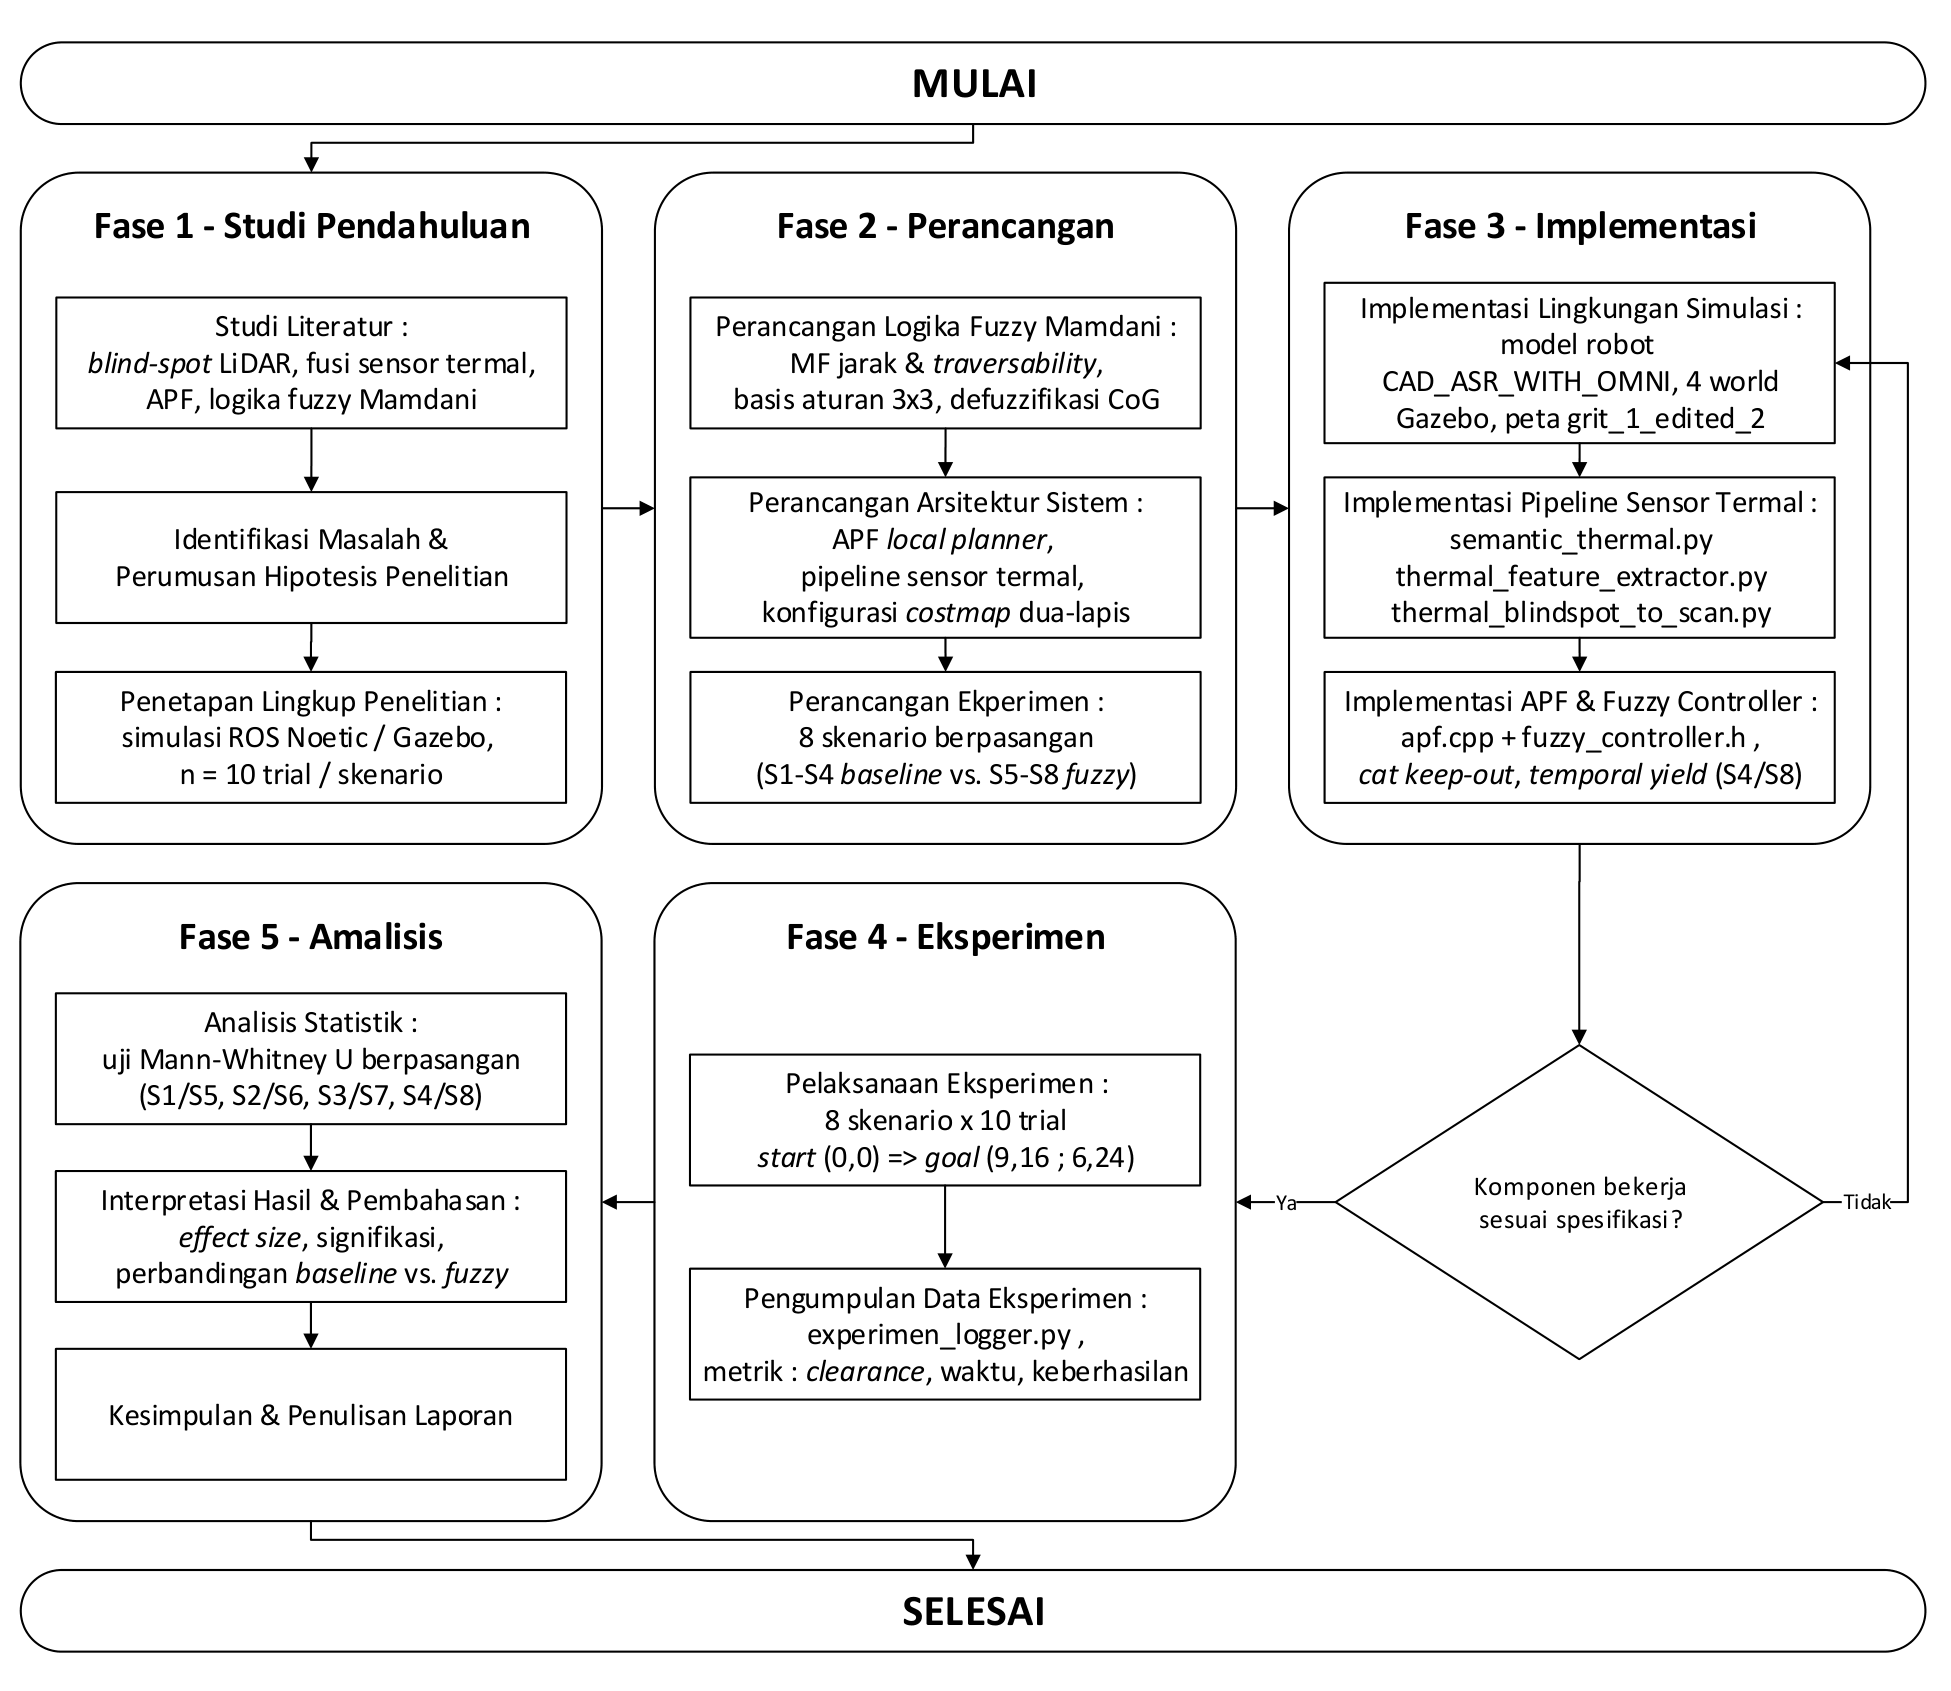
\includegraphics[width=\textwidth]{gambar/3.1_alur_penelitian.png}
\caption{Alur penelitian yang digunakan pada penelitian ini.}
\label{fig:alur_penelitian}
\end{figure}
